\chapter{Biodiversiteit}\label{ch:g5:biodiversity}

Neem één vierkante meter bloemrijke wei en begin te tellen: een stuk of
tien \omterm{def:g5:biodiversity:species}{soorten} \omterm{def:g1:plants-around-us:plant}{planten}, kevers en wantsen die niet te tellen zijn, spinnen,
slakken, wormen eronder en vlinders erboven. Probeer nu dezelfde
vierkante meter bestraat schoolplein. Het verschil tussen die twee
tellingen heeft een naam --- \omterm{def:g5:biodiversity:biodiversity}{biodiversiteit} --- en het is een van de
belangrijkste woorden van de \omterm{def:g1:living-or-not:living}{biologie} geworden.

\section{De verscheidenheid van het leven}

\begin{definition}[Soort]\label{def:g5:biodiversity:species}
Een \emph{soort}\index{soort} is één bepaald type \omterm{def:g1:living-or-not:living}{levend wezen}: alle
individuen die op hetzelfde model gebouwd zijn en die zich onderling
voortplanten. De huismus is een soort; het madeliefje ook, en de vos, en
de tuinslak. De klassen uit \cref{ch:g4:classifying-animals} zijn dozen
vol soorten: ``\omterm{prop:g3:sorting-living-things:groups}{zoogdieren}'' bevat er duizenden.
\end{definition}

\begin{definition}[Biodiversiteit]\label{def:g5:biodiversity:biodiversity}
De \emph{biodiversiteit}\index{biodiversiteit} van een plek is de
verscheidenheid aan leven die er te vinden is --- vooral: hoeveel
verschillende \emph{\omterm{def:g5:biodiversity:species}{soorten}} er leven, en hoe goed het elk ervan gaat.
Een bloemrijke wei, rijk aan \omterm{def:g5:biodiversity:species}{soorten}, heeft een hoge biodiversiteit; een
bestraat plein bijna geen.
\end{definition}

\begin{omfigure}
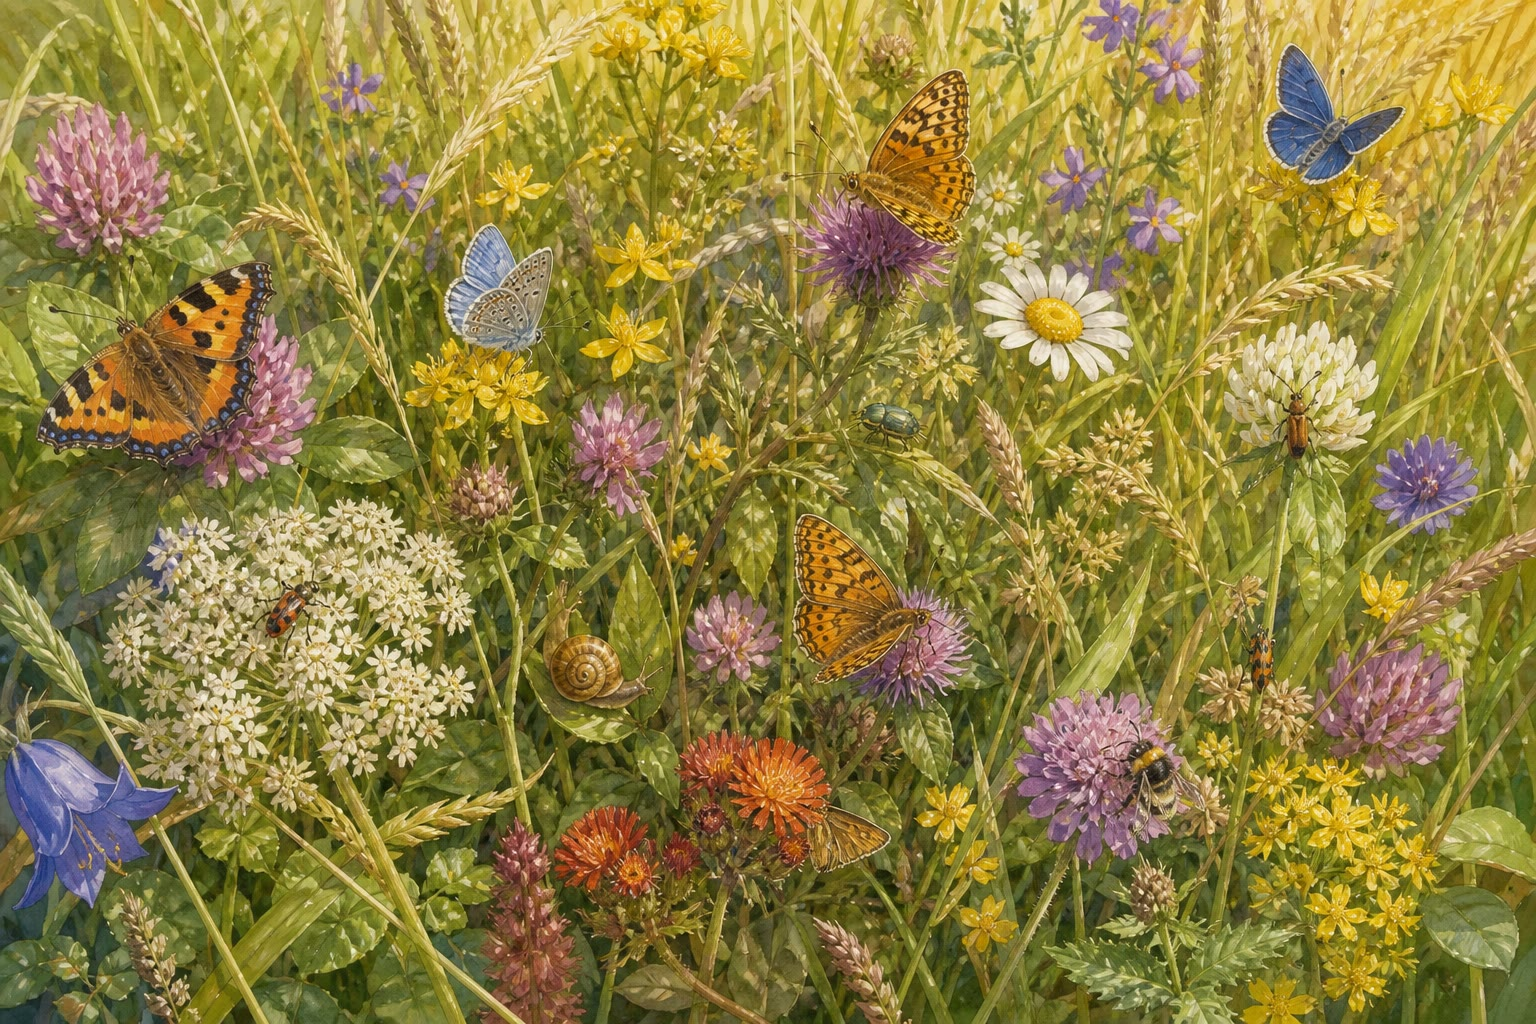
\includegraphics[width=0.62\linewidth]{images/book1/ai/g5-biodiversity-meadow.jpg}

{\small Eén vierkante meter wei, halverwege de telling: grassen,
\omterm{def:g3:flowers-fruits-seeds:parts}{bloemen}, vlinders, kevers, een slak --- en de telling is nog nauwelijks
begonnen.}
\end{omfigure}

\begin{example}[De planeet tellen]\label{ex:g5:biodiversity:planet}
Wetenschappers hebben tot nu toe ongeveer twee miljoen \omterm{def:g5:biodiversity:species}{soorten} benoemd
--- en ze weten zeker dat dat maar een deel van het totaal is, want elke
serieuze expeditie vindt nieuwe \omterm{def:g5:biodiversity:species}{soorten}: vooral kevers (geen groep heeft
meer benoemde \omterm{def:g5:biodiversity:species}{soorten}), maar ook \omterm{prop:g3:sorting-living-things:groups}{vissen}, kikkers, \omterm{def:g1:plants-around-us:plant}{planten} en zelfs af en
toe een zoogdier. Het volledige soortenaantal van de aarde is nog
onbekend --- de meeste schattingen lopen tot miljoenen boven wat benoemd is.
\end{example}

\begin{remark}[Verscheidenheid op elke schaal]\label{rem:g5:biodiversity:scales}
\omterm{def:g5:biodiversity:biodiversity}{Biodiversiteit} laat zich op meerdere schalen tegelijk zien: veel \omterm{def:g5:biodiversity:species}{soorten}
in één \omterm{def:g2:where-animals-live:habitat}{leefgebied}; veel verschillende \omterm{def:g2:where-animals-live:habitat}{leefgebieden} naast elkaar (vijver,
heg, wei --- elk met eigen \omterm{def:g5:biodiversity:species}{soorten}, zoals
\cref{ex:g2:where-animals-live:four} liet zien); en, binnen één \omterm{def:g5:biodiversity:species}{soort},
geen twee individuen helemaal gelijk --- geen twee tuinslakken dragen
precies hetzelfde huisje. Verscheidenheid binnen verscheidenheid binnen
verscheidenheid.
\end{remark}

\section{Waarom biodiversiteit ertoe doet}

\begin{proposition}[Het web heeft zijn draden nodig]\label{prop:g5:biodiversity:web}
De \omterm{def:g5:biodiversity:species}{soorten} van een \omterm{def:g2:where-animals-live:habitat}{leefgebied} voeden, beschutten, bestuiven en ruimen op
voor elkaar --- het zijn draden van één web
(\cref{rem:g3:food-chains:web}). Een rijk web met veel draden kan een
klap opvangen: als één prooisoort wegvalt, stappen haar jagers op andere
over. Een \omterm{def:g1:my-body:parts}{arm} web scheurt gemakkelijk: elke verloren \omterm{def:g5:biodiversity:species}{soort} laat de
overlevenden minder keuzes. \omterm{def:g5:biodiversity:biodiversity}{Biodiversiteit} is de sterkte van het web.
\end{proposition}
\admitted

\begin{example}[De boomgaardtest]\label{ex:g5:biodiversity:orchard}
Een boomgaard met heggen, bloemenstroken en oude bomen herbergt
tientallen helpersoorten: bijen en zweefvliegen bestuiven de bloesem
(\cref{rem:g3:flowers-fruits-seeds:bees}), lieveheersbeestjes eten de
bladluizen, \omterm{prop:g3:sorting-living-things:groups}{vogels} patrouilleren op rupsen, wormen houden de bodem open.
Rooi de heggen en maai de \omterm{def:g3:flowers-fruits-seeds:parts}{bloemen} weg, en de helpers vertrekken --- de
fruitteler moet hun taken dan alleen doen, taken die het web vroeger
gratis deed.
\end{example}

\begin{example}[Mensen leven van het web]\label{ex:g5:biodiversity:people}
Alles wat mensen eten is terug te voeren op levende \omterm{def:g5:biodiversity:species}{soorten}
(\cref{rem:g4:what-plants-need:everyone}); de meeste van onze medicijnen
zijn eerst in \omterm{def:g1:plants-around-us:plant}{planten}, schimmels en andere levende wezens gevonden;
katoen, wol, hout en leer zijn producten van \omterm{def:g5:biodiversity:species}{soorten}. De draden van het
web lopen dwars door elke keuken, apotheek en kledingkast.
\end{example}

\section{Biodiversiteit kan verloren gaan --- en geholpen worden}

\begin{proposition}[Hoe verscheidenheid verloren gaat]\label{prop:g5:biodiversity:loss}
Een \omterm{def:g5:biodiversity:species}{soort} loopt terug als haar wordt afgenomen waarvan ze afhangt:
\begin{itemize}
  \item haar \emph{\omterm{def:g2:where-animals-live:habitat}{leefgebied}} vernield --- de gedempte vijver uit
        \cref{prop:g2:where-animals-live:loss}, de gerooide heg, de
        bestrate wei;
  \item haar omgeving vergiftigd --- zwerfafval en chemische stoffen
        (\cref{prop:g2:caring-for-nature:harm});
  \item er te veel van weggenomen --- overbevist, overgeplukt,
        overbejaagd.
\end{itemize}
Een \omterm{def:g5:biodiversity:species}{soort} die helemaal verdwenen is --- overal, voorgoed --- is
\emph{uitgestorven}\index{uitgestorven}. Uitsterven is niet als een
verloren spel: er komt geen volgende ronde.
\end{proposition}
\admitted

\begin{method}[Biodiversiteit helpen, klein beginnend]\label{met:g5:biodiversity:help}
De recepten uit \cref{met:g2:caring-for-nature:rules} laten zich
opschalen:
\begin{enumerate}
  \item houd en \omterm{def:g1:plants-around-us:plant}{plant} verscheidenheid --- een heg van vijf struiken is
        beter dan een schutting, een bloemenstrook beter dan kaal grind;
  \item laat wilde hoekjes staan: dood hout, bladerhopen en ongemaaid
        gras zijn \omterm{def:g2:where-animals-live:habitat}{leefgebieden}
        (\cref{ex:g2:caring-for-nature:home});
  \item help de helpers: nestkastjes, insectenhotels, een vijver hoe
        klein ook
        (\cref{ex:g2:where-animals-live:schoolpond});
  \item tel wat er om je heen leeft, jaar na jaar --- wat geteld wordt,
        wordt opgemerkt, en wat opgemerkt wordt, wordt beschermd.
\end{enumerate}
\end{method}

\begin{example}[De terugkeer van de ooievaars]\label{ex:g5:biodiversity:storks}
Waar natte weiden hersteld werden en nestpalen werden opgericht, kwamen
ooievaars --- ooit uit hele streken zo goed als verdwenen --- terug om
te broeden, en met hen kikkers, libellen en weidebloemen. \omterm{def:g5:biodiversity:species}{Soorten} keren
terug als hun draden opnieuw geknoopt worden: bescherming werkt, en het
resultaat is vanaf het dorpsplein te volgen.
\end{example}

\section{Oefeningen}

\begin{exercise}[$\star$]\label{exo:g5:biodiversity:1}
Wat is een \omterm{def:g5:biodiversity:species}{soort}? Geef drie voorbeelden uit dit hoofdstuk.
\end{exercise}

\begin{exercise}[$\star$]\label{exo:g5:biodiversity:2}
Wat is \omterm{def:g5:biodiversity:biodiversity}{biodiversiteit}? Vergelijk de wei en het bestrate plein.
\end{exercise}

\begin{exercise}[$\star$]\label{exo:g5:biodiversity:3}
Ongeveer hoeveel \omterm{def:g5:biodiversity:species}{soorten} zijn er tot nu toe benoemd? Waarom is het
werkelijke aantal beslist hoger?
\end{exercise}

\begin{exercise}[$\star$]\label{exo:g5:biodiversity:4}
Noem de drie schalen van verscheidenheid uit
\cref{rem:g5:biodiversity:scales}, elk met haar voorbeeld.
\end{exercise}

\begin{exercise}[$\star$]\label{exo:g5:biodiversity:5}
Waarom overleeft een soortenrijk web klappen beter dan een \omterm{def:g1:my-body:parts}{arm} web?
Gebruik het argument van de jagers die op andere prooi overstappen.
\end{exercise}

\begin{exercise}[$\star$]\label{exo:g5:biodiversity:6}
Noem vier helpersoorten van de boomgaard en de gratis taak die elk doet.
\end{exercise}

\begin{exercise}[$\star$]\label{exo:g5:biodiversity:7}
Geef de drie manieren waarop een \omterm{def:g5:biodiversity:species}{soort} terugloopt, met bij elk een
voorbeeld. Wat betekent \emph{\omterm{prop:g5:biodiversity:loss}{uitgestorven}}?
\end{exercise}

\begin{exercise}[$\star$]\label{exo:g5:biodiversity:8}
Probeer het: tel de \omterm{def:g5:biodiversity:species}{soorten} --- \omterm{def:g1:plants-around-us:plant}{planten} en \omterm{def:g1:animals-around-us:animal}{dieren}, benoemd of beschreven
--- in één klein vierkantje dat je buiten uitkiest. Tel daarna ter
vergelijking een bestraat vierkantje. Jouw twee getallen zijn een meting
van \omterm{def:g5:biodiversity:biodiversity}{biodiversiteit}.
\end{exercise}

\begin{exercise}[$\star\star$]\label{exo:g5:biodiversity:9}
``Eén keversoort van de duizenden verliezen kan er niet toe doen.''
Antwoord met \cref{prop:g5:biodiversity:web} --- en met het feit dat
niemand alle draden kent die een \omterm{def:g5:biodiversity:species}{soort} vasthoudt.
\end{exercise}

\begin{exercise}[$\star\star$]\label{exo:g5:biodiversity:10}
Het ooievaarsverhaal heet een succes van \emph{\omterm{def:g2:where-animals-live:habitat}{leefgebied}}bescherming
en niet van ooievaars één voor één beschermen. Leg het verschil uit met
\cref{prop:g2:where-animals-live:loss} en met wat er naast de ooievaars
terugkwam.
\end{exercise}

\begin{exercise}[$\star\star\star$]\label{exo:g5:biodiversity:11}
Een boomgaardhouder vervangt heggen en bloemenstroken door schuttingen
en grind, en moet daarna bijenkasten huren voor de bestuiving en spuiten
tegen bladluizen --- geld uitgeven aan taken die eerst gratis gedaan
werden. Leg met \cref{ex:g5:biodiversity:orchard} uit wat er werkelijk
weggehaald is --- en waarom de rekening van het gratis werk van de natuur
meestal pas opduikt als dat werk ophoudt.
\end{exercise}
